\documentclass[11pt]{amsart}
%\usepackage{geometry}                % See geometry.pdf to learn the layout options. There are lots.
%\geometry{landscape}                % Activate for for rotated page geometry
%\usepackage[parfill]{parskip}    % Activate to begin paragraphs with an empty line rather than an indent
\usepackage{graphicx}
\usepackage{amssymb}
\usepackage{epstopdf}
\pagestyle{plain}
% -------------------- this stuff for code --------------------
\usepackage{color}
\usepackage{listings}

\usepackage{afterpage,lastpage,fancyhdr}
\usepackage[includeheadfoot,margin=2.5cm]{geometry}
\geometry{letterpaper}                   % ... or a4paper or a5paper or ... 

%\lstset{ %
%language=MATLAB                % choose the language of the code
%basicstyle=\footnotesize,       % the size of the fonts that are used for the code
%numbers=left,                   % where to put the line-numbers
%numberstyle=\footnotesize,      % the size of the fonts that are used for the line-numbers
%stepnumber=1,                   % the step between two line-numbers. If it is 1 each line will be numbered
%numbersep=5pt,                  % how far the line-numbers are from the code
%backgroundcolor=\color{white},  % choose the background color. You must add \usepackage{color}
%showspaces=false,               % show spaces adding particular underscores
%showstringspaces=false,         % underline spaces within strings
%showtabs=false,                 % show tabs within strings adding particular underscores
%frame=single,           % adds a frame around the code
%tabsize=2,          % sets default tabsize to 2 spaces
%captionpos=b,           % sets the caption-position to bottom
%breaklines=true,        % sets automatic line breaking
%breakatwhitespace=false,    % sets if automatic breaks should only happen at whitespace
%escapeinside={\%*}{*)}          % if you want to add a comment within your code
%}
% -------------------- end of code stuff --------------------



\DeclareGraphicsRule{.tif}{png}{.png}{`convert #1 `dirname #1`/`basename #1 .tif`.png}

\title{Machine Learning Decision Trees Coursework}
\author{Jean Kossaifi (jk712, a5) \\Sedef Ozlen (so512, s5) \\Paul Gribelyuk (pg1312, a5) \\Romain Brault (rb812, a5)}
%\date{}                                           % Activate to display a given date or no date

\begin{document}
\maketitle
\section{Summary}
We implemented the decision trees algorithm via modular, object-oriented approach to allow flexibility when testing and modifying the algorithm.  This also allowed us to split the work between the team members and used GitHub for version control.  
The workhorse class responsible for representing the tree is defined recursively as a node, which has "kids", i.e. child nodes, which, in turn, represent subtrees of the tree.  We store the information gain and the depth of the node in the tree, which we later used in the decision-making algorithm when the tree classifier gave ambiguous results.  The project is split up into the following files:
\begin{itemize}
\item[-] \emph{ID3Driver.m}: This function takes (i) examples, (ii) targets, (iii) attributes (as column indices), (iv) a decision function, (v) and the number of folds to use for validation as inputs, and return the confusion matrix, $F_{\alpha}$, a classification rate, and the six binary trees (as an array of nodes).
\item[-] \emph{ID3.m}: This is the algorithm which learns the binary tree by processing the examples until leaf nodes are reached.
\item[-] \emph{tnode.m}: This is the object representation of a node in a tree.  It can have an arbitrary number of child nodes, as well as properties such as ig (information gain), op (node label), and indop (index into the attribute array that this node has split the data on).
\item[-] \emph{ChooseBestDecisionAttribute.m}: This function returns the attribute that splits the data along the lines of the maximal information gain.
\item[-] \emph{trainer.m}: This method is responsible for producing the 6 trees given a set of examples, attributes, and targets.
\item[-] \emph{binaryFromMultiple.m}: Simple method which takes in target data with multiple classifications and converts it to a binary classification.
\item[-] \emph{classify.m}: Given some trees, example data, and a decision function, this method returns an array of predicted classifications.
\item[-] \emph{igClassify.m}: Our decision function which classifies the example data based on the sum of the information gains down a tree when an ambiguous situation arises (i.e. when either more than one tree returns a positive answer, or when all trees return a negative answer).
\item[-] \emph{depthClassify.m}: Another decision function we devised which resolves ambiguities based on shortest depth in the case of more than one positive answer, and longest depth in the case of all negative answers.
\item[-] \emph{NFoldValidationMask.m}: This is a helper function which returns 2 masks of "count" data points, for training and testing "N" times.
\item[-] \emph{ConfusionMatrix.m}: This method takes in predicted and actual target data and returns a confusion matrix.
\end{itemize}

\section{Tree Diagrams}
\begin{figure}[h]
\begin{center}
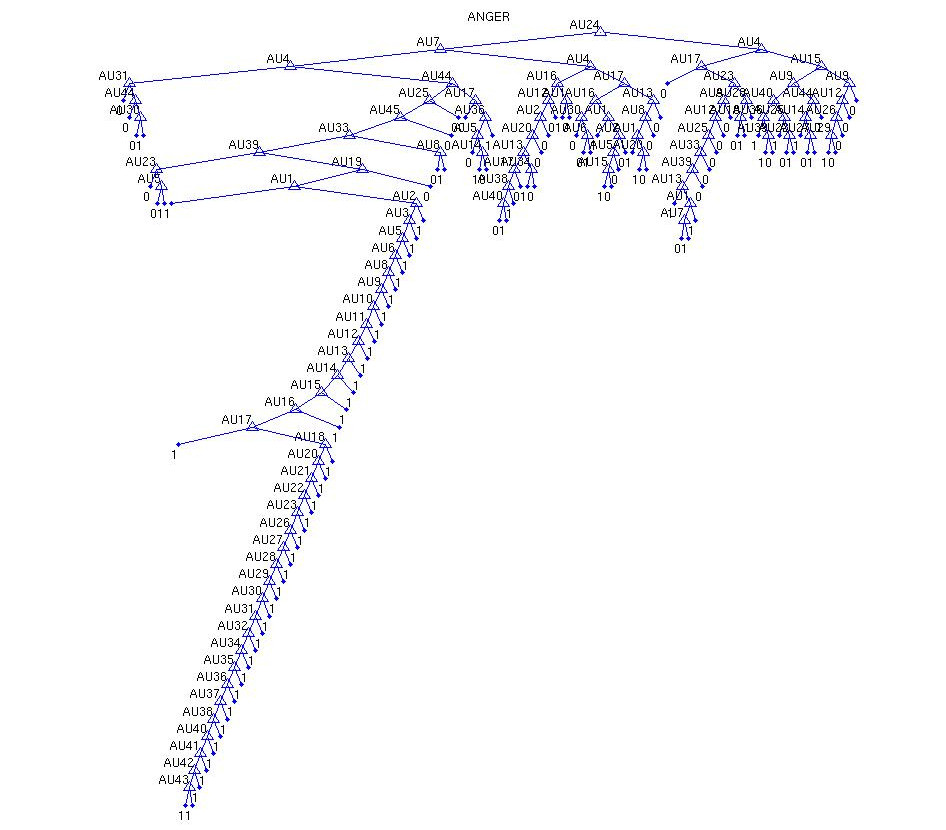
\includegraphics[scale=0.4]{anger.jpg}
\end{center}
\end{figure}

\begin{figure}[!h]
\begin{center}
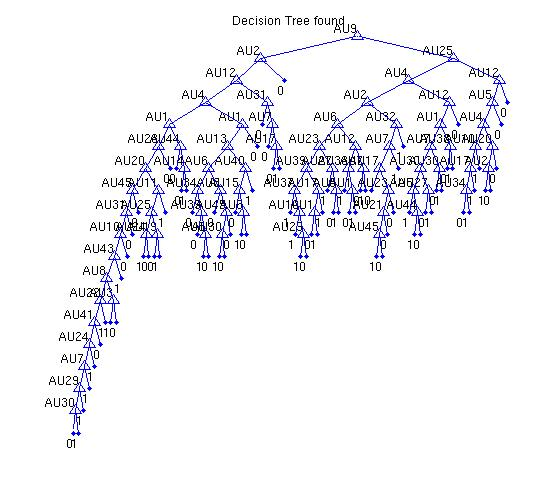
\includegraphics[scale=0.7]{disgust.jpg}
\end{center}
\end{figure}

\begin{figure}[!h]
\begin{center}
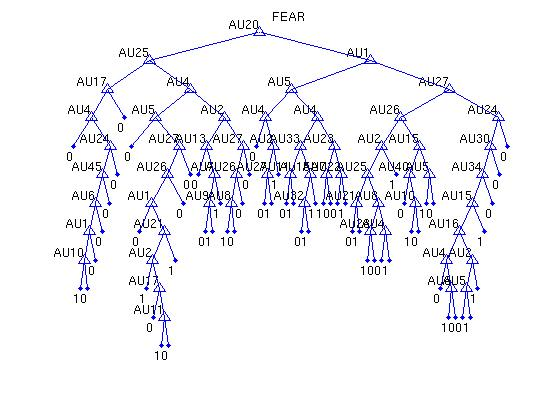
\includegraphics[scale=0.6]{fear.jpg}
\end{center}
\end{figure}

\begin{figure}[!h]
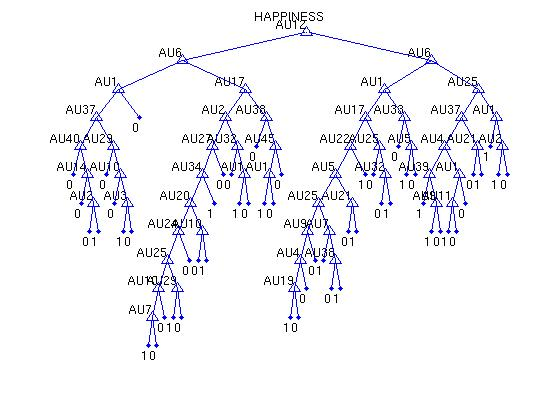
\includegraphics[scale=0.6]{happiness.jpg}
\end{figure}

\begin{figure}[!h]
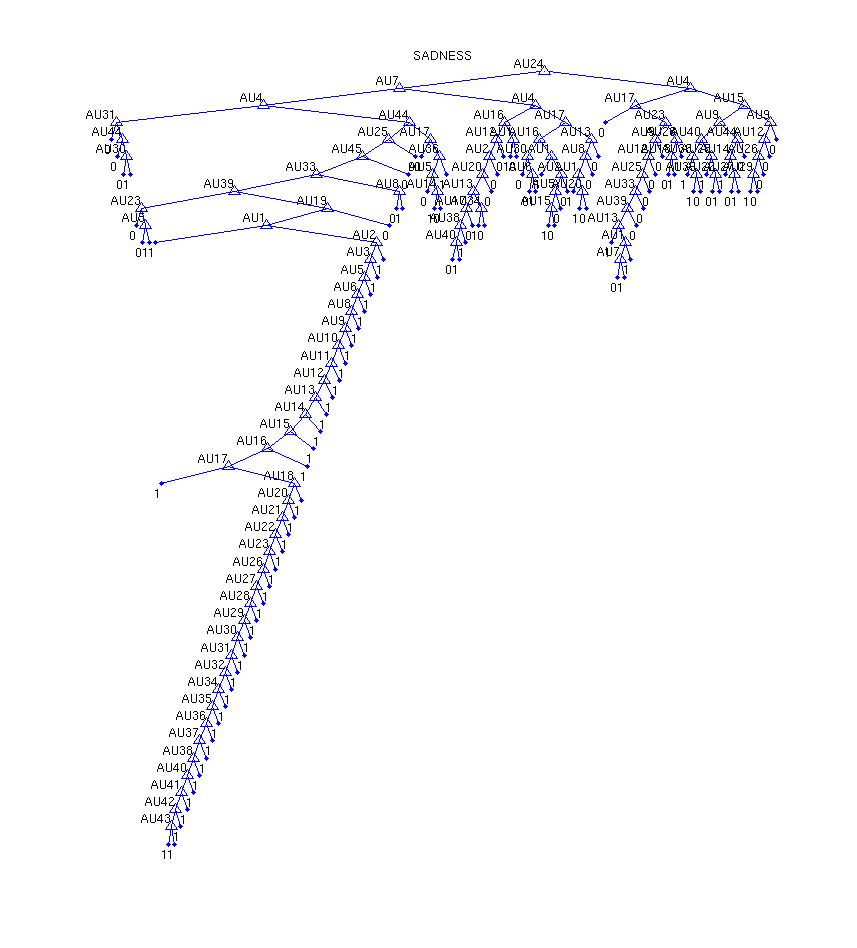
\includegraphics[scale=0.6]{sadness.jpg}
\end{figure}

\begin{figure}[!h]
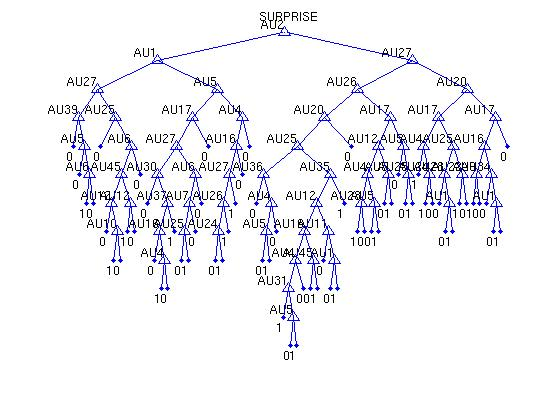
\includegraphics[scale=0.6]{surprise.jpg}
\end{figure}
\clearpage

\section{Results}
To obtain the results, we run the following code:
\begin{lstlisting}
[cm, err, cr, tr] = ID3Driver(x, 1:45, y, @igClassify, 10);
\end{lstlisting}
The confusion matrix is:
$$
cm = \left[\begin{array}{cccccc}
9.7000   & 9.7000 &   0.5000 &   0.1000 &   1.7000    &0.2000 \\
    1.9000   &15.1000&    0.1000&    0.6000&    1.4000 &   0.6000 \\
    1.2000    &0.7000    &8.4000    &0.2000    &0.5000   & 0.9000 \\
    0.5000    &1.4000    &0.4000   &17.7000   & 0.7000   & 0.8000 \\
    2.6000    &1.4000    &0.6000    &0.6000    &7.6000    &0.3000 \\
    0.2000    &0.5000    &1.8000    &0.6000    &1.0000   &16.5000 \\
\end{array}
\right]
$$
Furthermore, we obtained $F_{\alpha} = 73.4\%$, $classRate = 24.6\%$.

    

\section{Resolving Ambiguity of Tree Selection}
The ambiguity about deciding which binary decision tree to use arises whenever more than one tree returns a positive result or when all trees return a negative result (otherwise, the unique tree which returns a positive classification can be used to make the overall classification).  We first decided to handle these cases based on the aggregate information gain accumulated (additively) when walking down the tree in search of the result.  Our reasoning was that the tree which most clearly divides the data (and thus has the highest cumulative information gain) is more likely to be classifying the emotion.  This turned out to have a better effect than randomly selecting a tree (we obtained $F_{\alpha} \approx 70\%$ and $classError \approx 27\%$ via this method ($F_{\alpha} \approx 75\%$ and $classError \approx 22\%$).  
Our second approach was to resolve the ambiguity by selecting the shortest path which gave a positive result among all positive results.  If two paths are of the same length, then the selection resorts to a random one.  If no trees return a positive result, then we select the one which took the longest to traverse to our "no" answer.  Our rationale for this is that we can have the most confidence in the shortest path (which yielded a negative classification), those the longest one should result in the most error-prone answer, thus a "no" is more likely to be a "yes".  We believe that the longer path of a tree is likely the result of noise or overfitting, thus we ascribe less confidence to its prediction.
One of the advantages of the depth-based classification decision is that we can avoid the extra overhead of storing data at each node in each tree while we are building it.  However, we believe that the information gain approach produces better results because the maximal information gain could help produce the correct result even when there is some noise further down the tree.  For example, if happiness is described by AU12, AU6, and AU25, then an addition of another action unit to the example could produce a false negative in the answer, but the information gain could be large because the first three action units are very common to the happiness class.  Overall, we believe these approaches work in a similar way, but the information gain has more predictive power.
\section{Analysis of Tree Pruning}


\section{Code Flowchart}
%\subsection{}



\end{document}  